\section{The resilience polyhedron and certified protection design}
\label{sec:optimization}
The target antichain converts a continuum of spatial failure opportunities into a finite family of cuts. We now use that family to design a protection allocation. The cost model is explicit: allocating a nonnegative value $c_i$ makes deletion of contact $i$ cost $c_i$ to the adversary, and providing that protection consumes $d_i c_i$ units of resource, where $d_i>0$.\footnote{A linear hardening law is a mathematical engineering model. A physical deployment needs an experimentally justified map from protection resource to attack or failure cost. The paper does not infer that law from sensor geometry.}

\subsection{Concavity and weakest-point certificates}
Equation \cref{eq:kappa} shows that $\kappa_T$ is a finite minimum of linear forms. It is concave, positively homogeneous and coordinatewise nondecreasing on $\R_{\ge0}^n$. A minimizing cut $A$ supplies both an attack and a supergradient:
\begin{equation}\label{eq:supergradient}
\kappa_T(c')\le\kappa_T(c)+\boldsymbol1_A\cdot(c'-c).
\end{equation}
Indeed, the right side is $c'(A)$, one of the values over which $\kappa_T(c')$ takes its minimum. At a tie, any convex combination of the tied cut vectors is also a supergradient. The geometric witness associated with the chosen cut identifies where that adversarial value is attained.

Define the fractional blocking polyhedron
\begin{equation}\label{eq:blocking-polyhedron}
\mathcal B_T=\{z\in\R_{\ge0}^n:z(A)\ge1\text{ for every }A\in\mathcal A_T\}.
\end{equation}
For $\tau>0$, the condition $\kappa_T(c)\ge\tau$ is equivalent to $c/\tau\in\mathcal B_T$. This is the standard fractional transversal formulation of a cut hypergraph, here with exact geometric witnesses on the constraints.

\subsection{Primal and dual protection programs}
For a total protection budget $C\ge0$, the best guaranteed deletion cost is
\begin{equation}\label{eq:primal-protection}
\begin{aligned}
V_T(C,d)=\max\ &t\\
\text{subject to }&t\le\sum_{i\in A}c_i\quad(A\in\mathcal A_T),\\
&\sum_i d_i c_i\le C,\qquad c_i\ge0.
\end{aligned}
\end{equation}
The number of cut constraints is bounded quadratically in the geometric input size. This does not make all sensor-placement or wiring problems linear programs: positions and domain assignments remain separate variables in different models.

\begin{theorem}[Protection duality and exact certificates]\label{thm:protection}
The value of \cref{eq:primal-protection} is
\begin{equation}\label{eq:dual-protection}
V_T(C,d)=C\min_{\lambda\in\Delta(\mathcal A_T)}
\max_i\frac{\sum_{A\ni i}\lambda_A}{d_i},
\end{equation}
where $\Delta$ is the probability simplex on the antichain. In particular, if $c\ge0$, $d\cdot c\le C$, $\lambda_A\ge0$, $\sum_A\lambda_A=1$ and
\begin{equation}\label{eq:dual-feasible}
\sum_{A\ni i}\lambda_A\le\mu d_i\quad\text{for every }i,
\end{equation}
then
\begin{equation}\label{eq:certificate-interval}
\min_A c(A)\le V_T(C,d)\le C\mu.
\end{equation}
If the two displayed bounds are equal, these data constitute an exact optimality certificate.
\end{theorem}
\begin{proof}
For any primal-feasible allocation and any dual-feasible pair,
\[
\min_A c(A)\le\sum_A\lambda_Ac(A)
=\sum_i c_i\sum_{A\ni i}\lambda_A
\le\mu\sum_i d_i c_i\le C\mu.
\]
This proves weak duality and the certificate assertion using only finite sums and inequalities.

For equality of the optimal values, assume $C>0$ and put $x_i=d_i c_i/C$. Unused budget can be assigned to any coordinate without decreasing any cut sum, so $x$ can be restricted to the simplex. The normalized value becomes
\[
\max_{x\in\Delta_n}\min_{A\in\mathcal A_T}
\sum_{i\in A}\frac{x_i}{d_i}.
\]
The finite minimax lemma proved in \cref{app:minimax} exchanges this maximum and minimum after the adversary randomizes over cuts. The inner maximum over $x$ is the largest coordinate $\sum_{A\ni i}\lambda_A/d_i$, giving \cref{eq:dual-protection}. For $C=0$, both sides are zero. The feasible sets are compact after normalization, so optima are attained.
\end{proof}

The dual vector is a distribution over weakest target patterns, not a model of the actual failure distribution. Its purpose is to prove that no allocation under the stated resource budget can exceed the certified value. The coordinates $\lambda_A$ can be rational when the input is rational, and equality in \cref{eq:certificate-interval} is then checkable by integer arithmetic.

\begin{corollary}[Fractional transversal interpretation]
If $\varnothing\notin\mathcal A_T$, let
\[
\tau_T^*(d)=\min\{d\cdot z:z\in\mathcal B_T\}.
\]
Then $V_T(C,d)=C/\tau_T^*(d)$. If the antichain contains the empty cut, $V_T=0$.
\end{corollary}
\begin{proof}
For a desired value $t>0$, scaling \cref{eq:blocking-polyhedron} shows that the least resource cost is $t\tau_T^*(d)$. Solving $t\tau_T^*(d)\le C$ gives the formula. If the empty cut occurs, every allocation has $c(\varnothing)=0$.
\end{proof}

\subsection{Duplicating contacts and a sharp budget distinction}
Suppose each original contact $i$ is replaced by $b_i\ge1$ independently labeled copies with exactly the same footprint. Each target cut is expanded by replacing $i$ with all its copies. Under unit deletion costs this can increase the number of required deletions substantially. Under a fixed linear protection budget it has a different effect.

\begin{proposition}[Duplication invariance for the stated protection model]\label{prop:duplication}
If every copy of contact $i$ has the same unit protection coefficient $d_i$ as the original, duplication leaves $V_T(C,d)$ unchanged after aggregating copy allocations. This statement concerns the adversarial linear-cost model, not independent failure probabilities.
\end{proposition}
\begin{proof}
Given copy allocations $c_{i,j}$, put $\bar c_i=\sum_jc_{i,j}$. Every expanded cut has cost $\sum_{i\in A}\bar c_i$, and the budget is $\sum_i d_i\bar c_i$. Thus every copy allocation has exactly the value of a feasible original allocation. Conversely every original allocation is realized by putting its entire $c_i$ on one copy and zero on the remaining copies. Both optimization problems have the same feasible aggregate values.
\end{proof}

The four-corner panel and its duplicated eight-contact version illustrate the distinction. Their minimum numbers of individual deletions are two and four, respectively, but their unit-budget optimal protection values are both $1/2$. Independent Bernoulli reliability can still improve after duplication. A design comparison must specify which of these objectives is being optimized.

\subsection{Numerical proposals and rational verification}
The implementation may ask a floating-point LP solver for a candidate allocation and dual multipliers. It then converts proposed rationals, enforces nonnegativity and budget feasibility, normalizes the dual distribution, and sets $\mu$ to the largest exact ratio in \cref{eq:dual-feasible}. It computes both bounds of \cref{eq:certificate-interval} using rational arithmetic.

Only exact equality establishes verified optimality. If rational recovery yields a gap, the valid conclusion is the interval in \cref{eq:certificate-interval}. Solver status alone is never a proof. The allocations in the analytical examples below are derived symbolically with matching dual bounds, so their optimality does not depend on a numerical optimizer.

\begin{figure}[!htbp]
\centering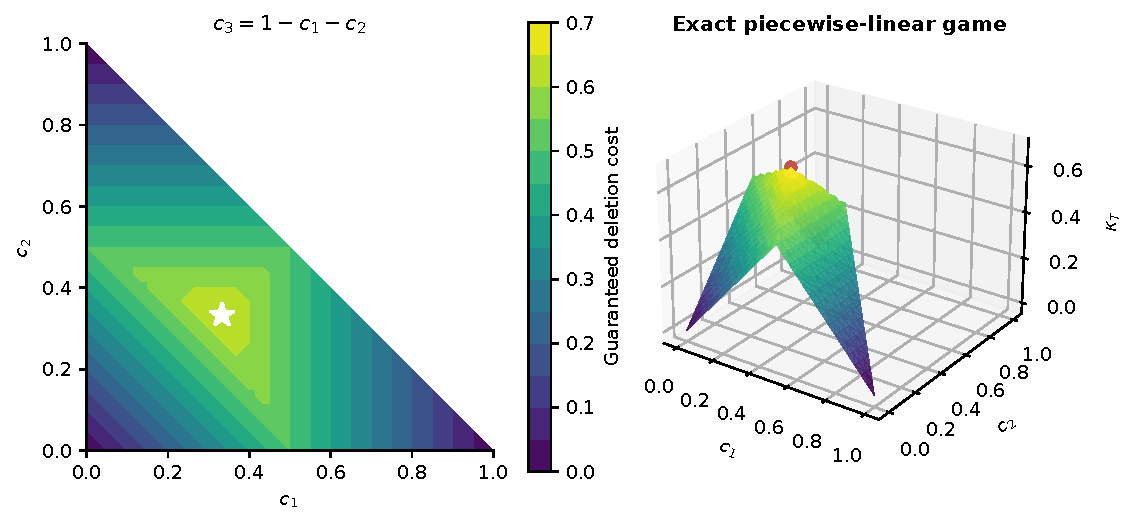
\includegraphics[width=\textwidth]{figures/budget-game.pdf}
\caption{Protection design for the three-asset example. On the unit simplex, $\kappa_T(c)=1-\max_i c_i$. The surface is piecewise linear and attains $2/3$ at the balanced allocation. The diagram displays the exact formula; numerical plotting does not determine the optimum.}
\end{figure}

\FloatBarrier
